\chapter{Introduction}

[tbd]

\begin{itemize}
	\item Explain structure and main goal of this thesis
	\item Introduction Chapter: Describe shortly all sections from this chapter and what the reader can expect
	\item Give short outlook to following chapter
\end{itemize}


% ---------------------------------------------------------------------------------------------------------
% ---------------------------------------------------------------------------------------------------------


\section{E-Commerce}


% [Internet]
\subsection{The Internet}

In the last 50 years, a new technology emerged, spread over the entire world and influenced many aspect of most peoples life.
Within the turmoil of the cold war, the United State's Advanced Research Projects Agency (ARPA) established in 1957 a communication network to bring together universities and their researches all around the country in order to be able compete against the USSR (\cite{2011Cohen}). % cite 2011 COhen
What started as a tool for scientific collaboration evolved a half century later into the internet, a global network and phenomenon, to which every user with a dedicated device has access and can contribute to.
The internet is an integral part, if not the backbone of today's everyday life.
Users of the internet use it for everything, that is sending emails, watching television, chatting with friends, 
order lunch, checking the weather for the next day or renting motorized scooters.

% [Numbers]

In 2021, the internet has 4.66 billion users, which is around 60\% of the world population.\footnote{Following statistics are taken from \url{https://datareportal.com/reports/digital-2021-germany} [14.05.2021]}
Compared to 2020, the number of internet users increased by 7.3\%.
In Europe, more than 90\% of the population are also internet users.
For a developed country like Germany, the numbers are even more impressing:
94\% of the German population are using the internet with an average daily time of over 5h.

Those numbers demonstrate impressive that the internet is an integral part of our daily life.
Along the rise of internet users, transactions and processes falling under the term of e-commerce rise.
Before discussing the term "e-commerce" and take a grasp at its history and types, some statistics are presented to demonstrate the importance of e-commerce.


% [E-Commerce]
\subsection{E-Commerce}

\subsubsection{Introduction}

From the global data report, we can see that over 90\% of the world population visited an online retail site.
Over 76\% of the world population purchased a product online.
For most categories growth is over 15\%.
Again, for a western country like Germany, the numbers are higher:
92.5\% of the german population visited an online retail site and over 80\% purchased a product online.
And the usage is growing: growth of amount spent in category food and personal care is 28.6\%, and 17.6\% for fashion and beauty.

Revenue in e-commerce is constantly growing over the last 20 years, topping to 57.8 billion in 2019.\footnote{\url{https://einzelhandel.de/presse/zahlenfaktengrafiken/861-online-handel/1889-e-commerce-umsaetze} [14.05.2021]}

% [Corona: Even more growth]

The COVID-19 pandemic with its implications had and still has an not negligible impact on the growth of e-commerce.
Several measures were taken to stop the spread of the virus and the number of deaths, one of which was to minimize physical interaction between people.
This leads consequently to a shift of human interactions to the internet.
Along this, e-commerce benefits.
Bhatti et al. (\cite{2020Bhatti}) conclude that "e-commerce enhanced by COVID-19".

% [E-Commerce History]
\subsubsection{Short History}

E-Commerce, or electronic commerce, is according to the \textit{Encyclopædia Britannica} about "maintaining relationships and conducting business transactions that include selling information, services, and goods by means of computer telecommunications networks."\footnote{\url{https://www.britannica.com/technology/e-commerce} [19.05.2021]}
In short, e-commerce is about buying and selling products and services via the internet.

% TODO check for Tian when paper available:
The success of e-commerce is tightly coupled to the vast advances of internet technology in the past years, like for example the development of the Electronic Data Interchange (EDI) starting from the 1960s, which standardised the communication between two machines.

Personal computers in 1980s and one of the first examples of online shopping is from CompuServe who introduced Electronic Mall in 1984.

Another milestone is Word Wide Web, introduced in 1990 by Tim Berners-Lee, made internet accessible to everyone.
First browser by Tim.

Social media since 2000 again offeres new possibilities for businesses and consumers alike to participate in e-commerce, e.g. for marketing, selling channels

New devices such as smart phones and tablets again decreases the hurdle to participate in e-commerce.
While in the time dimension e-commerce was already available all the time, with the new mobility its also available everywhere.
More flexible.
\cite{2019Hermogeno}.

With the ongoing progress in technology, also e-commerce can expect a shining future with trends such as AI recommendation systems, outstanding UX thanks to Virtual Reality, simple payment methods with crypto etc.\footnote{\url{https://www.spiralytics.com/blog/past-present-future-ecommerce/} [19.05.2021]}


% [Types]
\subsubsection{Types}

Multiple types in e-commerce are existing. They emerge from the possible combinations between the actors \textit{business}, \textit{consumer} and \textit{government} (\cite{2017DosSantos}).

\begin{itemize}
\item B2B: Business to Business
\item B2C: Business to Consumer
\item C2C: Consumer to Consumer
\item G2C: Government to Consumer
\item B2G: Business to Government
\item G2G: Government to Government
\end{itemize}

% [B2C]
\paragraph{B2C}
Business to Consumer in e-commerce describes basically online shopping, by means of a business offering its services and products to the consumer over the World Wide Web.
The consumer can browse within an online shop through the presented products and services and order them directly via the website.
A variety of payment and delivery options conclude the B2C type (\cite{2020Heinemann}).
% cite Heinemann with correct page p. 75 ?

For a aspiring business, multiple ready to use software solutions to install an online shop are existing, for example. Shopify, ePages, Magento or WooCommerce (\cite{2019Steireif}).

% [Amazon]
A famous example of a B2C company is Amazon.
On the 16th of July in 1995, Amazon launched as a website and entered the stock market on the 15th of May 1997 (\cite{2019Stone}). % cite also that this is directly from page p. 47 ?
Amazon is successful, the stock started with a price of X, which is at the time of this writing at Y.\footnote{\url{https://finance.yahoo.com/quote/AMZN?p=AMZN} [19.05.2021]}
Today Amazon employs over 1 million employees\footnote{\url{https://www.statista.com/statistics/234488/number-of-amazon-employees/} [19.05.2021]} and serves the wishes of 200 million paying prime members.\footnote{\url{https://www.statista.com/statistics/829113/number-of-paying-amazon-prime-members/} [20.05.2021]}


% [Pro and Con]
By taking a quick look at the pros and cons of maintaining an online shop, we can see that some of the advantages are that there is no need of a real house to present and sell the products, the virtual shop is available to the consumer at any time and has to closing hours; there is a high potential for the online shop as it is part of growing market; online business is scalable; due to tracking algorithms precise targeting as well as data analysis is possible; to start with an online business, not that much float is needed and there are in general lower costs; it is possible to provide a personalized customer experience; 

Some disadvantages are that the speed of market is rapid, competitors arise everyday everywhere, technology evolves quickly while consumers expectations go high (\cite{2019Hermogeno}, \cite{2020Lang}).


% [Performance of online shop is important]
Another downside is that there is no direct or physical concat with the consumer.
As described above, online shopping takes place in the World Wide Web domain.
Consequently, in person interaction between a buyer and a seller is not possible and the shopping event takes place on a website.
Deriving from this fact, the overall virtual user experience needs to be outstanding in order to stay ahead of competition.
The performance of the online shop is one part of the user experience.

In the next section, I will describe the findings between the correlation between user satisfaction and the performance of the retailers web presence.



% ------------------------------------------


\subsection{User Satisfaction and Performance}

% [User Satisfaction]
The aim of this thesis is not to deep dive into terms and concepts or the non-trivial problem of defining user satisfaction, usability or the like.
Therefore the term user satisfaction is in this context loosely defined as how happy the user is with the website he or she interacts with.\footnote{For a discussion cf. "User satisfaction measurement" in } %cite 2010 Islam

% [Performance]
For this context, performance can be understood as the the speed of an online shop, e.g. how long it takes the page to load, how quickly the user can interact with the page, and how the user perceives the performance of the website.
Later we will see that measuring performance is not that trivial and a lot of ideas and metrics are existing to measure it.


% [SpeedHub]
\subsubsection{SpeedHub}

A plethora of information and studies about the phenomenon of user satisfaction and web site performance is collected at \textit{SpeedHub.org}, a portal by \textit{Baqend} in cooperation with \textit{Google} which provides "the largest systematic study of Mobile Site Speed and the Impact on E-Commerce."\footnote{\url{https://www.speedhub.org/} [21.05.2021]}
On the hub, not only studies and reports are available, but also collections of videos and blog posts.

% [code.talks 2019]
In his presentation at code talks 2019, Felix Gessert summarizes the findings and provides insights to the most relevant aspects and questions of the study so far: %cite 2019 Gessert

% [User Profile and Psychology]
The first observation when tackling the question regarding a correlation between the performance of a system and the user satisfaction, is that the users have to be distinguished which leads to the concept of a \textit{User Profile}: Regarding gender, young woman are the most demanding consumers and buy less on slow pages.
Generally, people between 18 and 24 have higher expectations regarding site speed than their older counterparts.

There are also differences between nations and regions, for example people from Japan have the highest expectations, which for a certainty coheres with the technological progress in this country.
Not only the expectations themselves differ geographically, but also how speed influences the users, for example "speed influences New Yorkers more than Californians."

% cite 
% Think Fast, The 2019 Page Speed Report Stats & Trends for Marketers, Unbounce, 2019
% Brain Food, Speed Matters, Designing for Mobile Performance, Google, 2017


What all users have in common is their human psychology. With respect to performance, researchers generally suggest to keep waiting times under 1000 ms in order to keep the users attention.
% cite
% I. Girgorik, High performance browser networking, O'Reilly Media 2013
% Jakob Nielsen, Usability Engineering, Morgan Kaufmann, 1994

% [Devices]
After considering the user itself, the next step is to investigate the influence of the device in use: Studies show that mobile users are more likely to buy products and services than their colleagues using a desktop computer, where iOS users have generally more expectations regarding site speed.
% cite
% Android vs iOS market share 2019 Q2. DeviceAtlas, 2019.
 
% [Context]
Last but not least is the context and the users condition important, where naturally relaxed and calm users perceive sites faster than stressed users or people that are in a hurry.
Also when on the move, users experience sites slower.
% cite Performance Matters. 9 Key Consumer Insights, Akamai, 2014.


% [Studies]
There are many real world examples and studies existing which prove and demonstrate the importance of site speed with respect to user satisfaction and eventually revenue:
\textit{Amazon} fount out that a decrease of 100 ms in page loading leads to -1\% conversion rates.
If the site loads 100 ms faster, \textit{Walmart} observed that the revenue increases by 1\%.
For \textit{Zalando}, increasing site speed by 100 ms leads to an uplift of 0.7\% revenue per session.
% cite
% Greg Linden. Make Data Useful. Standford Data Mining Class CS345A, 2006.
% Shuhei Kagawa, Jeff Cybulski, David Martin Jones, et al.. Landing Time Matters. Zalando Tech Blog, 2018
% C. Crocker, A. Kulick, B. Ram. Real-User Monitoring at Walmart. SF & SV Web Performance Group, 2012

% [SEO]
Search Engine Optimization is heavily impacted by load speed:
For \textit{Google}, 500 ms slower sites lead to a decrease of 20\% in traffic.
\textit{GQs} traffic increased by 80\% after the page load went down from 7 s to 2 s.
And for \textit{Pinterest}, 40\% faster loads led to 15\% more SEO traffic.
% cite
% Lucia Moses. How GQ Cut Its Webpage Load Time By 80 Percent. Digiday, 2015
% Marissa Mayer, Conference Keynote, Web 2.0, 2006.
% Sam Meder, Vadim Antonov, Jeff Chang. Driving User Growth With Performance Improvements, Pinterest Blog, 2017



% [Engagement & Satisfaction]
Also the user engagement and satisfaction rely heavily on load times:  \textit{Forrester} noted an increase of 60\% for the session length while brining down the load time by 80\%.
\textit{Akamai} monitored that the bounce rate climbed up incredible 103\% when the load time increased by 2 seconds.
And for the \textit{AberdeedGroup}, the customer satisfaction dropped by 16\% at one more second delay in response times.
% cite
% Forrester. The Total Economic Impact Of Accelerated Mobile Pages, 2017.
% Akamai, Akamai Online Retail Performance Report: Milliseconds Are Critical, Akamai Blog, 2017
% The Performance of Web Applications: Customers Are Won or Lost in One Second. Aberdeen Group, 2008.



To summarize, many studies and real world examples prove and demonstrate that faster web sites and online shops cause a better user experience and typically lead to happier customers. 
Concluding in commercial terms, one can say with a certainty that page speed equals money.
\\

In order to properly test the impact of performance on the users, a scientific method is needed.
A/B testing as a controlled experiment is one of them and will be explained in the next section.
After a discussion of A/B Testing, I will move on to the examination of \textit{Web Analytics}, a term which subsumes methods, tools and instruments for businesses to better understand their business and customers.


\subsubsection{A/B Testing}

% 2012 Kessler 17.2  AB Tests ?


% 2016 Kohavi
Controlled experiments such as A/B Testing are not a new tool for scientists and researchers and have been used already in the 1920s. % cite Kohavi 2016
With the rise of the internet in the 1990s, the concept has been adopted to the online domain and is as of today widely used by big companies such as Amazon, Facebook or Google to directly test ideas and hypothesises on a live system.
Controlled experiments such as A/B Testing are utilised to support decision making and to deliver "causal relationship with high probability". % cite Kohavi 2016
They enable a data driven and quantitative validation of the hypothesis. % cite Morys 2018

Controlled experiments help to test hypothesis and questions of the form: "If I change feature X, will it help to improve the key performance indicator Y?"

To answer this question,  two systems are needed: Version A, the control variant or default version, and a slightly different version B, called the treatment.
If more than two versions or one treatment should be evaluated at the same time,  an A/B/n split test has to be implemented.
For an univariable setup, only one variable differs between the systems, where in a multivariable structure, more than one variables are changed at the same time.

Usually, the users of the system are randomly split into two groups and testing is directly performed with real users on a production system.
Beneficial, also when comparing with other experimental setups, is, that the users and participants are not aware that they are part of an experiment, which leads to less bias and side effects.
In order to measure the differences and the user behaviour, web analytics has to be integrated within the system.
% cite Kohavi 2016


% TODO write those steps down ?
% 2018 Morys
%- 5 steps:
%- 1. quality of hypothesis according to SOR Paradigma
%- 2. quality of testconcept: isolation and contrast of changed parameters
%- 3. quality of implementation and quality assurance: running tests should not be visible by user (e.g. suddenly UI changes) and performance of website should not be impacted
%- 4. quality of measurement: significant difference in primary goals
%- 5. quality of statistical interpretation: amount of data, statistical methods


A short and general discussion about controlled experiments in computer science is in chapter X. %link chapter about controlled experiments


% [Transition to Web Analytics]

To resume with the question of performance and user satisfaction,  A/B testing enables to serve two different versions of the same site to two groups, one site being slow, the other one fast, at the same time without the users knowing.
With web analytics implemented, it is possible to measure how the different systems and user groups behave.

What web analytics exactly is, what tools are available and how a web analytics process looks like, will be discussed in the next section.




% Heinemann 2020 A/B Tests nach 4.1.4



% ------------------------------------------------------------------------------------
% ------------------------------------------------------------------------------------
% ------------------------------------------------------------------------------------
% ------------------------------------------------------------------------------------




\section{Web Analytics}

First some definitions, then quickly summarize the history, and then technical aspects of collecting data.


\subsection{Introduction}

% [Definitions]
What is Web Analytics?
Going through the literature, makes it clear that multiple definitions are existing:

Nakatani et al. state that "Web analytics is used to understand online customers and their behaviors, design actions influential to them, and ultimately foster behaviors beneficial to the business and achieve the organization's goal." % cite 2011 Nakatani
According to this definition, web analytics is about getting insights of the users using the system, not only who or what they are, but also how they interact with the system.
Additionally, the definition stressed that the underlying motivation of web analytics is are the achievement business goals.

Singal et al provide a more technical definition by pointing out that "Web Analytics is the objective tracking, collection, measurement, reporting and analysis of quantitative internet data to optimize websites and web marketing initiatives." % cite 2014 Singal with note that this definition is directly taken from Kaushik
Again, the ultimate target is to drive business forward, but backed up with data science methods and instruments such as tracking, collecting and analysis of vast amount of data.

Bekavac et al provide a similar definition by pointing out that web analytics is "the analysis of qualitative and quantitative data on the website in order to continuously improve the online experience of visitors, which leads to more efficient and effective realization of the company's planned goals." %cite 2015 Bekavac:

% TODO: where can i find this officially ?
% Official definition by WAA: the measurement, collection, analysis and reporting of Internet data for the purposes of understanding and optimizing Web usage.

% TODO add 2009 Waisberg? "Web Analytics can be defined as the act of increasing a website’s persuasion and relevancy to achieve higher conversion rates."

% TODO add Croll 2009? "Today, web analytics is a marketing discipline used to measure the effectiveness of communications strategies" p.83

Summarizing above definitions, we can see that web analytics is composed of two important aspects: A data driven, information focused and technical aspect of collecting and analysis data about the users, and a commercial perspective, which provides the main motivation of collecting the data beforehand, by setting business goals.


% [Use Cases]
Moving from the definitions to the practical domain, Zheng et al. describe four main use cases for web analytics:

% 2015 Zheng
% TODO write more here
\begin{itemize}
\item Improve overall design and user experience
\item Optimize for your business goals
\item Monitoring
\item Improve performance
\end{itemize}

Those use cases in the end also target to make customers more happy and increase revenue.


% [Challenges]
Web analytics is also difficult and there are some obstacles to avoid and challenges to tackle.

% 2019 Kumar
Kumar et al. describe the hurdles as follows:
Data science challenges:
Statistical methods are not yet sophisticated enough.
Collected data is heterogeneous and incomplete.
A lot of data is available (big data).
Analysis not fast enough.

Privacy: tbd




% ------------------------------------------


\subsection{Short History}

The history of web analytics can be described as its shift from an IT domain and technical log file analysis tool towards a sophisticated, polymorphic instrument for marketers.

% [For IT: Logs]
% TODO add somewhere: Log file analysis is discussed in greater detail in chapter X. %refernece chapter

Everytime a user requests an html file or another resource from the webserver, an entry in a dedicated log file is made by the server. %cite Singal 2014
The first log entries followed the Common Log Format (CLF) which provides rudimentary information such as the date, the HTTP status code or the number of bytes transmitted.
In 1996, the Extended Log Format (ELF) was introduced with more flexibility and information in mind.
Thanks to the standardized format of log files, software could be build to analyse the log files and present them in a user friendly fashion.
\textit{GetStats} was one of the first tools which generated statistics and user friendly output for analysts.
% cite Croll 2009 p 69
and in 1995, Dr. Stephen Turner created Analog, the first free log file analysis software.% cite Zheng 2015

% [Shift]

What was in the beginning mainly interesting for maintenance and IT personal who answered questions such as how many 404s occurred on the server, turned into a website information pool interesting for marketers.

With the increase in available information it came clear that the data can be used for more than just analysing the servers behaviour.
But log file analysis was not sufficient enough to get details about how users interact with the website.
Web analytics experienced a transformation from log analysis logging to user data tracking, analysis and reporting.

Croll describes the move of analytics from IT to marketing with three steps: %cite Croll 2009
\begin{enumerate}
\item JavaScript made log files redundant and also empowered marketers to maintain and implement their analytics solutions, unravelling their dependence from the IT department.
\item The introduced advertisement economy from search engines like Google led to a new focus for analysts on user attraction and conversion rates.
\item New cost models enabled the marketers to pay for the analytics service according to the websites traffic, instead of paying for hard- and software in advance. The expenses for analytics were therefore coupled with the websites traffic and ideally revenue.
\end{enumerate}


% [For Marketing: JS]

In 1990 the \textit{World Wide Web} kicked off and one of the first widely used browsers \textit{Mosaic} launched in 1993.
At the same time \textit{WebTrends} developed and released one of the first analytics software.
A lot more services followed, such as \textit{WebSideStory} in 1996 % cite Zheng 2015
or Quantified by Urchin in the same year.%cite croll 2009

The page tagging technique enabled the collection of not only technical data, but also business relevant information.
Visitors and their behaviour were the main concern and coined to questions such as: How is this user behaviour linked to a purchase? If a user buys shoes, will he also buy socks?
The development and implementation of Cookies enabled the identification of unique users.
Not only business related questions were asked and answered, but also investigations of performance and usability.
% cite 2009 Croll p. 69

More details about page tagging in chapter X.


% 2014 Singal
In 2003, Edwards, Eisenberg and Sterne founded the Web Analytics Association (WAA).
The WAA is brings together and supports all actors of web analytics such as users, marketers and IT specialists on an international stage.
Due to the digitalization and its all-embracing impact, WAA renamed itself to Digital Analytics Association (DAA), as the web is not the only domain where users leave their digital footprint.
% cite 2014 Singal

As already described in the above section, the numbers of participants and users of the internet are still increasing and all Fortune 500 companies operate websites, with Web Analytics as a centrepiece tool in marketing. %cite Kumar 2019

Some of the most established tools today are Google Analytics, Adobe SiteCatalyst, Webtrekk and Piwik. % cite Heinemann 2020 4.1.4

Google Analyitcs will be discussed in chapter X.

Zheng et al. identify several future trends for Web Analytics, such as mobile web and application specific analytics like video-, search-, learning- or social media analytics. %cite Zheng 2015


% TODO add Image: Genesis of Web Analytics (nice graphic) with WAA, DAA ? should remove then in-page analytics arrow
% TODO add somewhere Some methods about tool selection are described in chapter X.

% TODO next section will be about process


% ------------------------------------------



\subsection{Web Analytics Process}


Web Analytics can be described as a process, where as a rule the main goal is to increase revenue.
In literature, two main ideas and process flows are indicated, the first one being from the Web Analytics Association, and the second one derived from industries best practices.
They will be concisely described in this section.

What both processes have in common is that they aim for improving the website and consequently increase the business revenue.

\textit{Key Performance Indicators} (KPIs) are the ideal tool to instrument web analytics and they help to determine areas and room for improving.
They are an integral part and play a major role in any web analytics process as they provide an "in-depth picture of visitor behavior on a site". %cite 2009 Jansen ch. 6.2

KPIs can differ according to the business they operate it.
For commercial domains, common KPIs are conversion rates, average order or visit value, customer loyalty, bounce rate, and so on.% cite 2014 Singal
Defining the right KPIs and align them with the business goals is a crucial step in any web analytics process.

% 2015 Bekavac:  KPIs for commercial model: Ratio of new to returning visitors, percentage of new visitors, referring domains, search keywords/phrases, average order value, key conversion rates



\subsubsection{WAA Process Guide}

Web Analytics Association provides a nine step guide:% cite 2009 Jansen ch. 6.2
\begin{enumerate}
\item Identify key stake holders
\item define primary goals of website and prioritize them
\item identify most important site visitors
\item determine key performance indicators
\item Identify and Implement the Right Solution
\item Use Multiple Technologies and Methods
\item Make Improvements Iteratively
\item Hire and Empower a Full-Time Analyst
\item Establish a Process of Continuous Improvement
\end{enumerate}



\subsubsection{Industries Best Practices}

Waisberg and Kaushik derive from industries best practices a five step process with the main goal, improve website, increase revenue, in mind:% cite 2009 Waisberg

\begin{itemize}
\item Define Goals
\item Build KPIs
\item Collect Data
\item Analyze Data
\item Implement Changes
\item Repeat last two steps
\end{itemize}
% TODO add graphic instead of list


% [Comparison]
Comparing both proposed processes, it is evident that both put the identification and awareness of the main business goals upfront.
WAAs process is are more fine grained and practical approach, where as Waisberg and Kaushiks flow abstracts the principal activities.


% ------------------------------------------



\subsection{Data Collection/Sources: Log Analysis versus Page tagging}

There are four main ways to collect data for web analytics: Logs, JavaScript Tagging (or page tagging), web beacons and packet sniffing. %cite 2009 Waisberg

As already mentioned in chapter X,  the two main data collection methods are Log file analysis and Page Tagging.
In this section, I will briefly describe both mechanisms and compare them to each other.


\subsubsection{Log File Analysis}

As already described in the above section X, log file analysis is about getting insights from the web servers log files records.

Log file analysis is considered to be the traditional and original approach to web analytics. %cite 2011 Marek and 2015 Zheng

Once the users enters a URL in the browser and hits enter, the request arrives at some web server.
The server then creates an entry in a log file and sends back the requested page or resource as a response to the client. % cite % 2009 Waisberg

The information within the log entry can vary depending on the log format, mostly provided are the IP, browser, timestamp, time taken, bytes transferred, whether a cache hit occured and the referrer. %cite 2009 Waisberg

The standardized Common Log Format provides host, ident, authuser, date, request, status, bytes, as seen in example X. \footnote{\url{https://www.w3.org/Daemon/User/Config/Logging.html\#common-logfile-format} [03.06.2021]}

\begin{center}
\begin{lstlisting}[caption={Position 1}, language=bash, numbers=none, basicstyle=\tiny]
127.0.0.1 user-identifier frank [10/Oct/2000:13:55:36 -0700] "GET /apache_pb.gif HTTP/1.0" 200 2326
\end{lstlisting}
\end{center}
% TODO add caption

Standard formats of log files and entries allow log file analysis software to process, evaluate and report valuable statistics to users, such as Analog, Webalizer or AWStats. %cite 2015 Zheng


% [Pro]
Following are lists describing the advantages and disadvantages of log file analysis.

Advantages of log file analysis are:

\begin{itemize}
\item JavaScript and Cookies are not required on the client side
\item Maintainer of the website and server owns the data %cite 2009 Waisberg
\item Bots and web crawler requests are also logged %cite 2009 Waisberg
\item History of data is available %cite 2011 Nakatani
\item Log entries are reliable %cite 2011 Nakatani
\item The standard format of log files enables easy switching of analysis tools %cite 2011 Nakatani
\item The web server also logs failed requests %cite 2011 Nakatani
\item No modification on the web page needed %cite 2015 Zheng
\item Does not demand more bandwidth %cite 2014 Singal
\end{itemize}


% [Con]
Some disadvantages are:

\begin{itemize}
\item Log entries provide mainly technical information, which may not be very useful for user behaviour analysis. Business related metrics such as bounce rates are not available. % cite Marek 2011
\item Only direct requests from the client to the web server are logged: Any user interaction in the web browser, which does not fires a request, is not getting logged. Also responses from caches and proxies are not visible in the web servers log file. Only interactions with the web server are logged.%cite 2015 Zheng
\end{itemize}



% ------------------------------------------


\subsubsection{Page Tagging}

In a nutshell, page tagging describes the analytics method of including JavaScript on the web page, which collects data and sends it to an analytics server. %cite 2011 Marek
For this, JavaScript has to be included on every page which should be analysed. %cite 2009 Waisberg
Page tagging is the main method used in web analytics today. %cite 2015 Zheng

Croll provides a vivid graphic about the page tagging process which will be discussed here (fig. X). %cite Croll 2009

\begin{center}
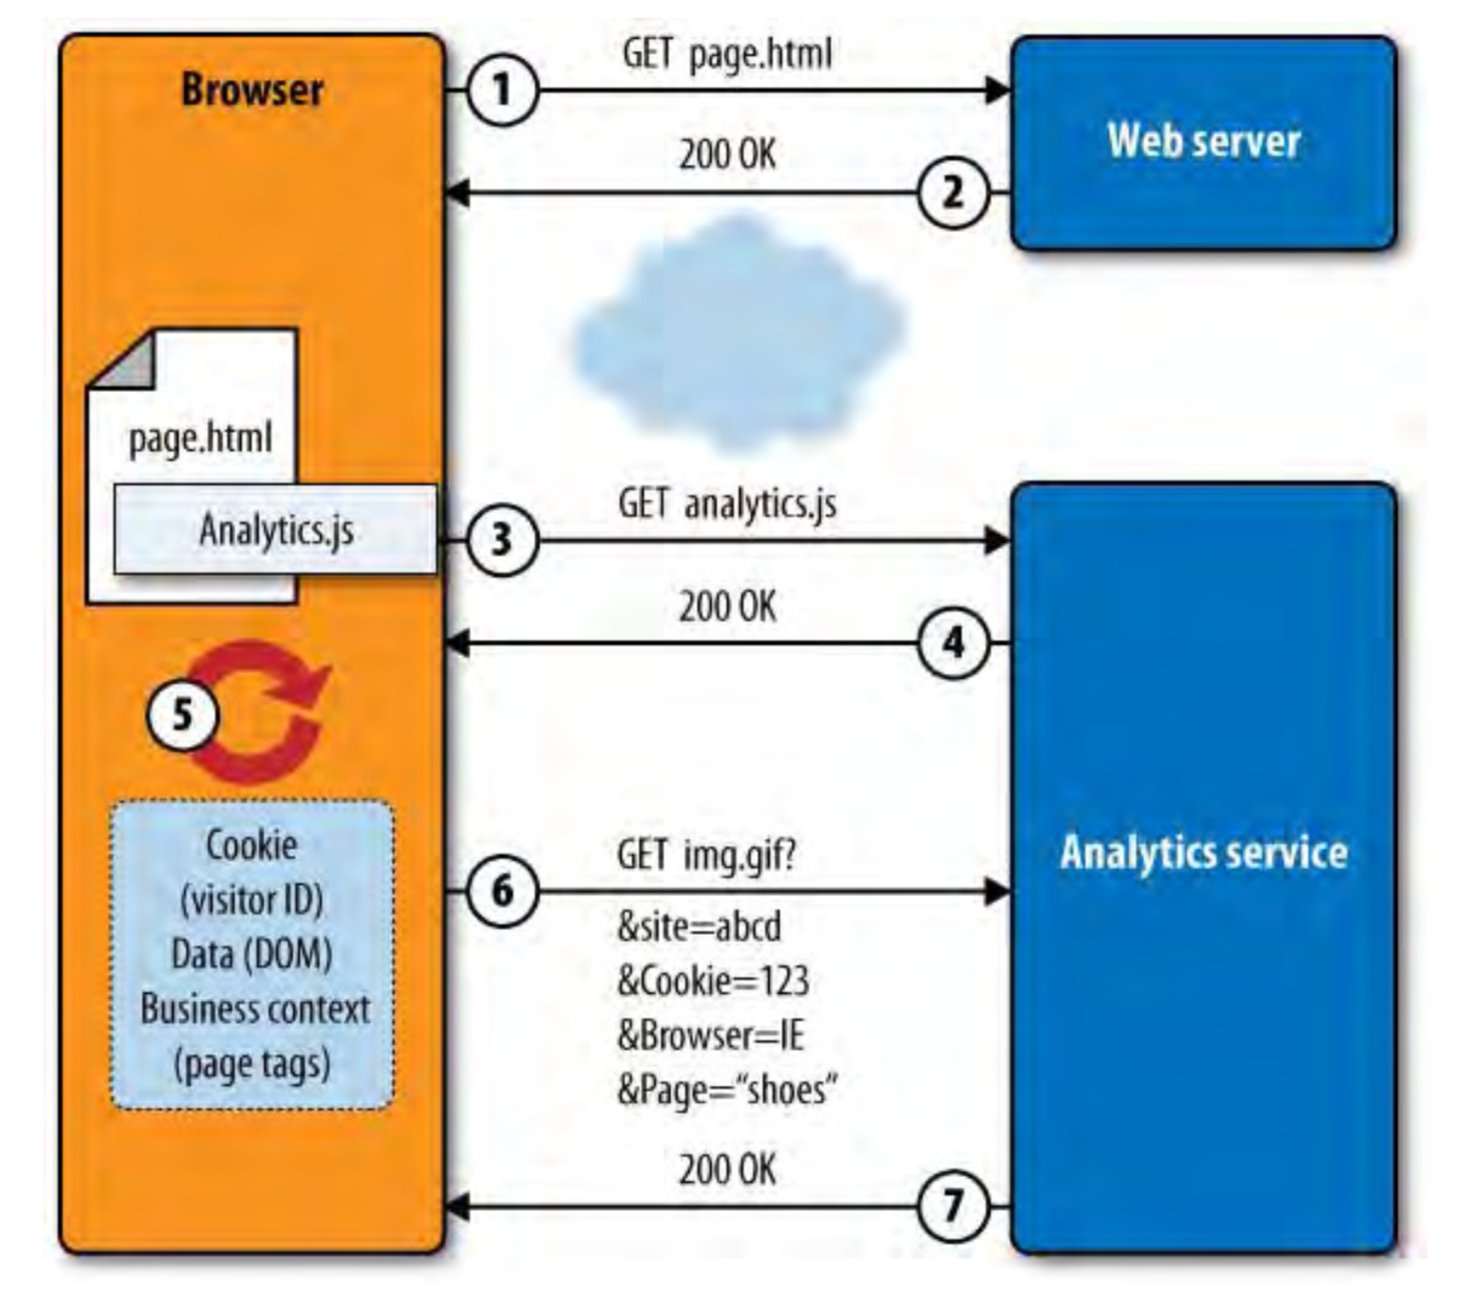
\includegraphics[width=0.5\textwidth]{page_tagging.png}
% TODO add caption
\end{center}

The client (browser) requests a page from the web server (1, 2).
Within the html file an external JavaScript resource, the analytics code, is linked and received from the analytics server (3, 4).
The analytics script tracks and measures the user behaviour and eventually sends the data back to the analytics server (5, 6, 7).

The collected data can also be stored in cookies, which persist data beyond one session and enable user identification, e.g. on his next page visit. %cite 2019 Kumar


The advantages and disadvantages of page tagging are as follows:

% [Pro]
\begin{itemize}
\item Every page visit is counted %cite 2009 Waisberg
\item The analytics service is outsourced, which includes the storage of the data, but also data analysis and reporting %cite 2009 Waisberg
\item Page tagging is rather easy to implement and favourable when the analyst does not have access to the web server %cite 2011 Marek
\item Highly customizable: anything that JavaScript allows to measure, collect and track is obtainable. This also includes information about the client such as screen size, device used or color depth. %cite 2011 Nakatani
\item Possibility to track events and actions such as mouse clicks that do not send requests to the web server. This is especially important for single-page or progressive web applications which do not fire requests that often. %cite 2011 Nakatani and 2015 Zheng
\item Mechanics of cookies provide identification of unique and repeat visitors %cite 2011 Nakatani
\item Real time reporting %cite  2014 Singal 
\end{itemize}



% [Con]
Some disadvantages are mainly privacy concerns, the analytics process relies on the usage of JavaScript and cookies which can be deactivated by the user %cite 2011 Marek
, every page which should collect data needs to include the analytics script, and due to the use of a third party analytics service it is rather difficult to switch tools. %cite 2014 Singal


% TODO 2017 Hassler ch. 2 ??

% TODO web beacons and packet sniffig ?
% 2011 Marek
% 2011 Nakatani
% 2014 Singal




% ------------------------------------------


\subsection{Web Performance}


\subsubsection{Introduction}

% [Definitions]

As already described in chapter X, web performance plays a non negligible role regarding user satisfaction and business success.
The cited studies demonstrate that increasing the websites performance also increases the revenue. 



% What is good performance ? -> Perceived performance
As seen in chapter X, everything below one seconds is good.
Thresholds for specific performance metrics and the psychological rationale of setting them will be discussed in chapter X.

Generally 

"A good goal for web performance is for users to not notice performance. "


% https://web.dev/why-speed-matters/
"Performance plays a major role in the success of any online venture"
"Performance is a foundational aspect of good user experiences. "



% https://developer.mozilla.org/en-US/docs/Learn/Performance/why_web_performance
- UX is subjective
"A good goal for web performance is for users to not notice performance. "
- financial aspect of downloading data and big websites



% https://developer.mozilla.org/en-US/docs/Learn/Performance/What_is_web_performance
- major areas:
- reducing overall load time
- Making the site usable as soon as possible
- Smoothness and interactivity
- Perceived performance
- Performance measurements


%  https://developer.mozilla.org/en-US/docs/Web/Performance
"Web performance is how long a site takes to load, become interactive and responsive, and how smooth the content is during user interactions"








Technical metrics which measure time stamps and UX. This will be discussed later in detail.
UX is in the end the truth.






% [Bottlenecks]

Why are websites slow?


% 2016 Witt
- the three bottlenecks: Frontend, network, backend



% 2013 Grigorik https://hpbn.co/primer-on-web-performance/
- Latency as a Performance Bottleneck







\subsubsection{Measuring Methods and Metrics}

Metrics in chapter X

Synthetic vs RUM

Practical example and experiment in chapter Z


% https://developer.mozilla.org/en-US/docs/Web/Performance/Rum-vs-Synthetic





% 2013 Grigorik https://hpbn.co/primer-on-web-performance/
- Synthetic and Real-User Performance Measurement



% 2021 Wolle blog post https://medium.baqend.com/mobile-site-speed-measurement-best-practices-ff4a3f91b003
- Log file
- Synthetic: will be discussed in chapter X
- RUM which will be covered in chapter X
- CrUX
- Surveys


% 2016 Kaur: Tools for Measuring the Performance of Websites
- Pingdom
- GTMetrix
- Website Grader
- Site Speed checker












% ---------------------------------------------------------------------------------------------------------------------------------
% ---------------------------------------------------------------------------------------------------------------------------------




\section{Research Question}

\begin{itemize}
\item Difficulty of defining scope
\item Measuring performance of a web site impacts its performance or other effects take place / Observer effect
\item Why the research question is relevant
\end{itemize}

What is the research question of this thesis?
What is the goal?

the intrinsic complexity of the field and the internet in general

% Measuring Real User Performance in the Browser: Avoiding the Observer Effect



Motivation


Goals of this thesis


\subsection{Chapter Outline}

This introduction chapter was about

In chapter X...

tbd











